% $Id: introduction.tex 65669 2015-01-09 14:55:20Z tgershon $

\section{Simulation}
\label{sec:Simulation}
It is crucial to any particle physics experiment to understand and be able to calculate the behavoiur of the detector and apparatus being used.  No detector is perfect, therefore only a fraction of the particles created in the process being studied actually get fully measured and reconstructued.  From this subset of detected particles one has to infer the total number of particles created and any relevant distributions related to the measurement in question, the only practical way to calculate these detector efficiencies is with a full detector simulation.  A full detector simulation is also crucial for detector performance studies, understanding backgrounds and comparisons between theory and experiment.

The complexity of particle physics detectors and the many degrees of freedom in the underlying problem behind a detector simualtion make it unfathomably complex and highly multi-dimensional.  Consequntly, the ``monte carlo''(MC) or statistical sampling method is used to perform these simulations due to the fact it deals with multi dimensinal problems very well and it makes the problem conceptually far easier to understand.  More specifically direct monte carlo is used.

The first step in the monte carlo simulation is the generation of a pp interaction.  This is the responsibility of the event generator, which generates particles with randomly generated properties sampled from the correct distributions.  In \lhcb \pythia is the defualt generator used for general purpose production, but \herwig++ is sometimes used as a cross check\cite{Sjostrand:2007gs,Herwig}.  Both of these generators also simulate the hadronisation of the particles created in the hard pp interaction but \herwig uses a cluster model and \pythia uses a string model.  There are also some specialised generators used which include: \bcvegpy for the production of \Bc mesons, GenXicc for \Xic production and Hiijing for heavy ion collisons \cite{bcvegpy,Gyulassy:1994ew,Chang:2007pp}.

The next stage of the simulation process is the transportation of the generated particles through the detector and all the interactions with the detector material that occur.  In \lhcb this is performed by the \geant toolkit which is a well established software framework solely created to simulate the interatctions of particles with matter \cite{Agostinelli:2002hh}.  It is this stage of the simulation process, as performed by \geant, that is the subject of study in this report.  \geant has the capability to simulate all relevant hadronic, electromagnetic and optical interactions in a wide energy range for many long lived particles. Futhermore, \geant manages the geometry of the apparatus being simulated and also has the capbaility to simulate magnetic fields that are present at all collider based particle physics experiments.

\geant was first commisioned in 1993 as a result of studies that looked at how modern computing techniques could impove the existing fortran based GEANT frameworks that date back to 1974\cite{Agostinelli:2002hh,Brun:118715}.  These studies lead to \geant being implemented as an object orientated framework in C++.  One of the many advantages of object orientation is the ease by which improvements and refinements to the existing code can be made.  Consequently, there are regular new releases of \geant, the latest version being 10.1\cite{g410.1rn}. However, this is yet to be implemented in \lhcb; until recently \geant v9.5.p02 was implemented in the \lhcb simulation package but this has recently been updated to v9.6.p04.  When a new release of \geant is adopted into the \lhcb simulation package it is important to validate the reuslts of the new package and understand any discrepancies compared to the previous version.  If changes to simulation results are not understood this could have series consequences for physics analyses due to the unavoidable reliance on simulation for detector efficiencies etc.  Part of the study presented in this report is a comparison of electromagnetic physics results between \geant version 9.5.p02 and version 9.6.p04 for two seperate scenarios, both of which are important to \lhcb.

The object orientated design of \geant means that it is very easy to have a variety of models avaiable for each interaction process; it is well known that the model giving the optimum agreement with data varies for different energy ranges and different particle types.  Consequently, it is important to be able to tailor the simulation to the specific scenario under investigation.  However, with the large number of interaction processes simulated and the large array of long lived particles to consider even a small selection of models for each process and particle would quickly lead to a very extensive range of possible configurations for the same scenario.  Therefore, \geant provides a set of physics lists (PL) each of which specifies a fixed set of models designed to be optimal for a smaller range of scenarios.  For example, there are PLs available for low energy scenarios which would specify models that show the best agreement with data at lower energy.  The effect of PL choice for scenarios relevant to \lhcb also forms part of the study detailed in this report.


\subsection{Simple Calorimeter Test}
\label{sec:Simple Calorimeter Test}
The first test to validate the new version of \geant  was an extended electromagnetic example designed to model an electromagnetic calorimeter.  The basic principle behind this comparison was to run this example within both \geant versions and compare selected results that could have implications for \lhcb.  

Firstly, checks were made to ensure that the implementation of the example was unchanged between versions to ensure any discrepencies could be attributed to changes global to the \geant framework and not just a change in this specific example.  After this had been established to be true, the example was setup to model the \lhcb electromagnetic calorimeter (ECAL) as closely as possible. As described in section \ref{sec:Detector}, the \lhcb ECAL is a sampling calorimeter consisiting of 66 alternating layers of lead and plastic scintillator \cite{LHCb-TDR-002}. In order to make this a direct comparison between what is currently implemented and what will be implemented the example was customised to run with the \lhcb private PL.  Therefore, the same physics models are being used in both versions, but the models themselves could have changed between versions.

\subsubsection{Fractional Resolution Investigation}
\label{sec:Fractional Resolution Investigation}

The first result used as a comparison tool between \geant versions was the fractional resolution of the electromagnetic calorimter.  No detector is perfect, therefore the energy of an incident particle is measured with a resolution defined by a gaussian distirbution.  However, the width of this gaussian distribution varies with the energy of the incident particle.  The fractional resolution is defined as $\frac{\sigma(E)}{E}$ where $\sigma(E)$ is the standard deviation of a particles measured energy at a given incident energy E.  The variation of the fractional resolution as a function of energy is given by, 
\begin{equation}\label{eq:fr}
\frac{\sigma}{E}=\frac{a}{\sqrt{E}} \bigoplus \frac{b}{E} \bigoplus c
\end{equation}
where a, b and c are constants to be defined\cite{wigmans2000calorimetry}.  

The 'a' term in equation \ref{eq:fr} arises from statistical fluctuations in the electromagnetic shower induced by the sampling calorimeter.  In an electromagnetic shower many particles are produced and the energy measured by the ECAL is the sum of the energies deposited by each particle.  However in a sampling calorimeter only a fraction of the shower takes place in active regions, therefore only a fraction of the shower particles are actually measured.  Consequently the number of shower particles that are measured is subject to poisson fluctutations with a standard deviation of $\sqrt{N}$, where N is the number of shower particles in the active region.  Assuming the calorimeter is linear (which it should be) the number of shower particles produced is proportional to energy, therefore $\frac{\sigma}{E} \propto \frac{\sqrt{N}}{N} \propto \frac{1}{\sqrt{E}}$. In a sampling calorimeter it is sampling fluctiations that dominate the resolution, thus the 'a' term is usually by far the largest term in equation \ref{eq:fr}.  

The 'b' term in equation \ref{eq:fr} arises due to electronic noise which causes energy independent resolution effects.  However, this is not simulated in this study and will therefore not be considered.  The 'c' term in equation \ref{eq:fr} arises due to shower leakage from the ECAL.  At a given energy the amount of energy lost from the ECAL is subject to event by event fluctuations, which leads to broadening of the resolution.  However, the total amount of energy lost from the ECAL is proportional to the energy of the incident particle and this dominates over the event by event effects.  This leads to the standard deviation of measured energies due to shower leakage being proportinal to incident energy, and consequently energy indpendent for the fractional resolution.

The first step towards obtaining the fractional resolution of the model ECAL was to fire electrons into the ECAL at several fixed energies.  At each energy a histogram was produced showing the distribution of energy deposited in active regions of the ECAL per event.  This distribution is predicted to be gaussian, therefore a minimum chi squared fit of a gaussian function was performed at each energy to obtain the mean and standard deviation of the distribution. An example of one of these fits is shown in figure \ref{fig:Gauss}.  This was performed at 13 different energies between 1.56GeV and 44.44GeV, this range was chosen because it includes the majority of electron energies expected at \lhcb.

\begin{figure}[h!]
  \centering
  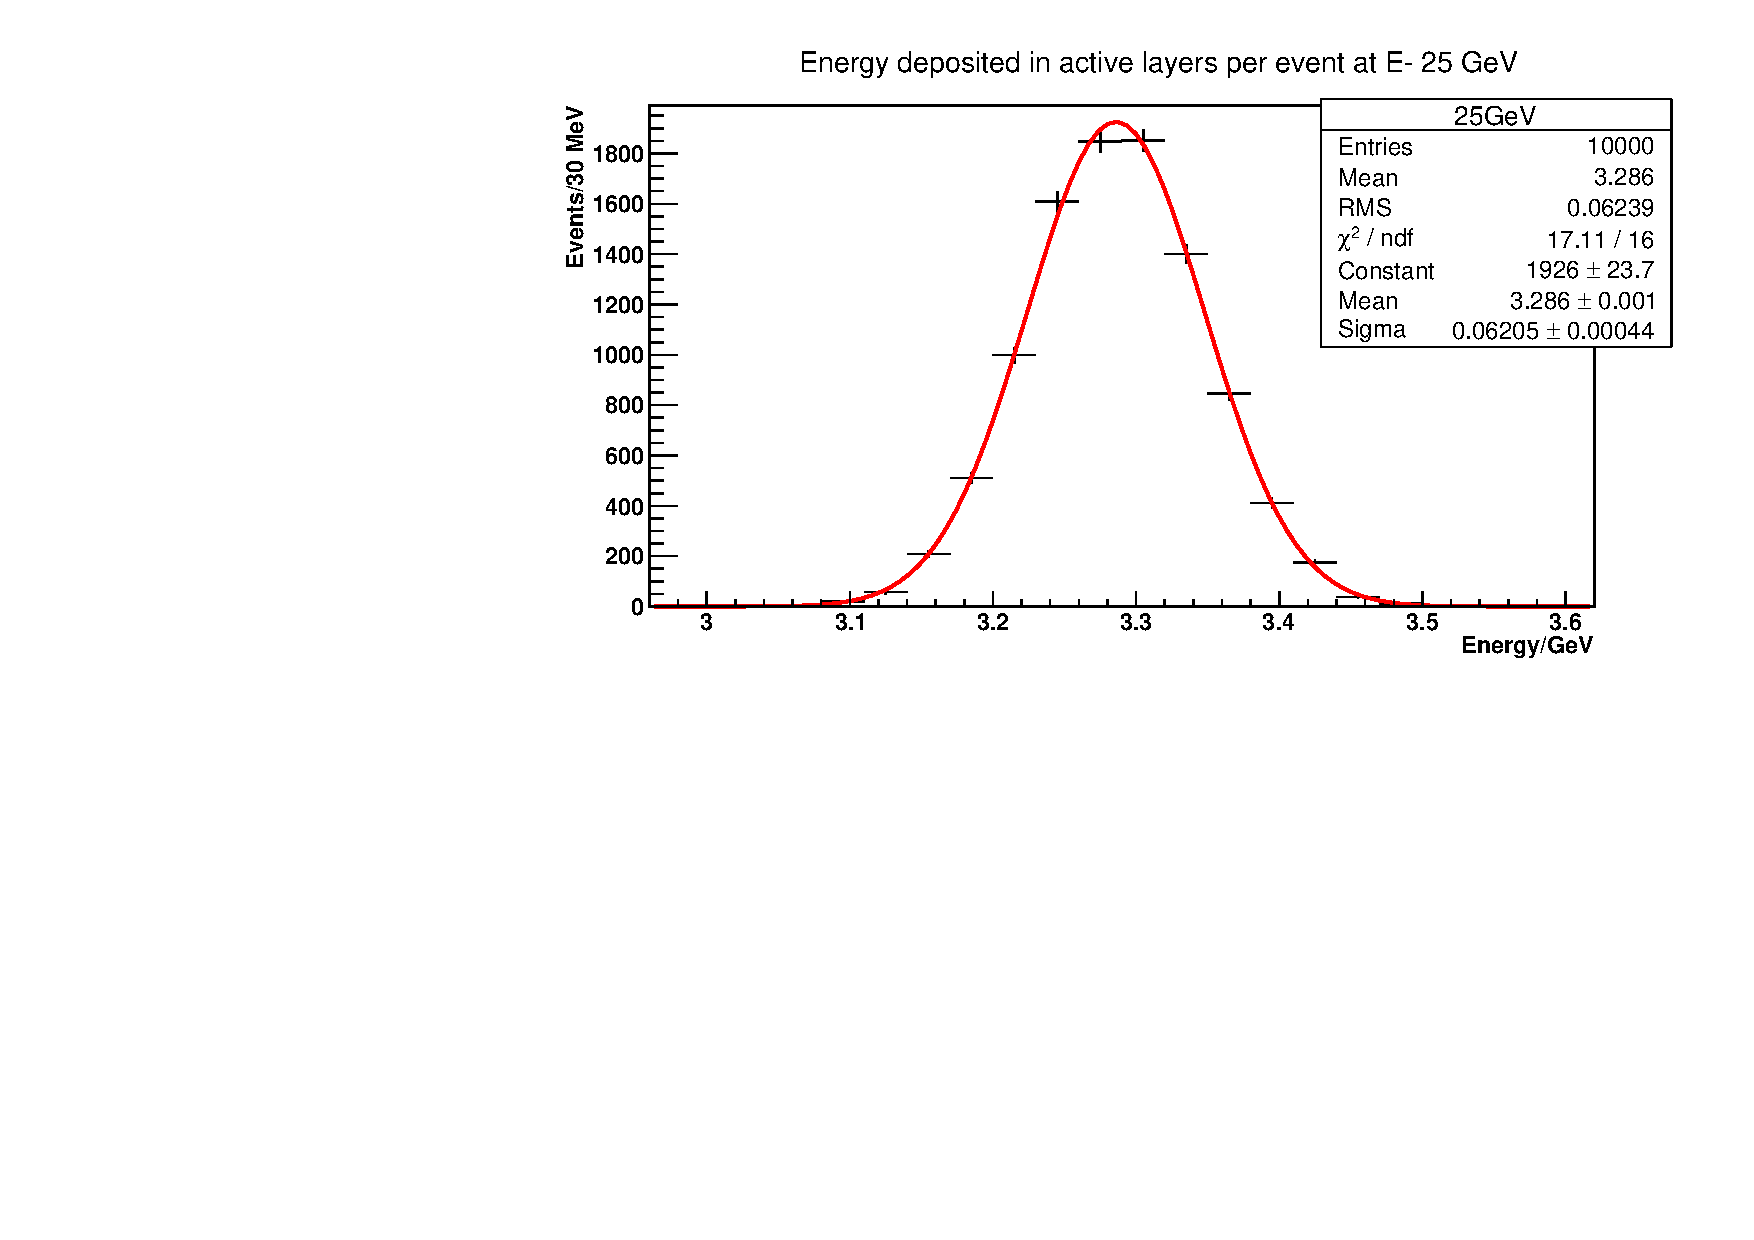
\includegraphics[width=\textwidth]{GaussExample.pdf}
  \caption{The distribution of energy deposited in scintillator(active) layers at 25 GeV}
  \label{fig:Gauss}
\end{figure}

From these fits the standard deviation divided by the mean was plotted against the incident particle energy, as defined in the configuration of \geant.  $\frac{\sigma}{E}$ is expected to follow equation \ref{eq:fr} but without the b term. Therefore a mimimum chi squared fit to,
\begin{equation}
  \label{eq:fitfr}
  \frac{\sigma}{E}=\frac{a}{\sqrt{E}}\bigoplus c
\end{equation}
was performed with the parameters 'a' and 'c' left floating as these are to be determined by the fit.  This process was applied to both \geant version 9.5.p02 and 9.6.p04 with the same energies and 10000 events at each energy.  The results of these fits for both \geant versions are shown in figures \ref{fig:straightres}, \ref{fig:coolres} and table \ref{tab:results}.

\begin{table}[h!]
  \centering
  \begin{tabular}{|c|c|c|c|}
      \hline
      Version: & v9.5 & v9.6 & Difference  \\ \hline
      A term    & 0.0952$\pm$0.0003 & 0.0922$\pm$0.0002  & 8.43$\sigma$, 3.3\% \\ \hline
      C term    & 0.0050$\pm$0.0003 & 0.0048$\pm$0.0003 & consistent \\ \hline
      $\frac{\chi^2}{ndf}$   &1.140  & 0.998 &  \\ \hline
  \end{tabular}
  \caption{Fractional resolution results for comparison of \geant versions}
  \label{tab:results}
\end{table}

It is clear from these fits that there is a significant discrepancy in the statistical term of the fractional resolution parameterisation between \geant versions, despite the same PL being used in both versions.  The simulation of electromagnetic showers is a well established process that, in general, shows good agreement with data.  Therefore, progression of results this significant is not expected.  As many different processes contribute to electromagnetic showering more investigations were needed to understand exactly which part of the simulation is giving rise to this discrepancy.




%Frac Res Investigation
%----Comparison of Geant4 versions
%Sampling fraction investigations
%----Comparison of Geant4 versions
%Physics List investigations
%----Fractional Resolution
%----Sampling Fraction Results

%MSC
%--results


